% Crucial Preamble
\documentclass[12pt,letterpaper]{article} \usepackage{amsmath} \usepackage{graphicx}  \usepackage{longtable}  \usepackage{amssymb}
%\usepackage[margin=0.7in]{geometry}

\usepackage[left=1.3cm,top=2.5cm,right=1.3cm,bottom=2.5cm,bindingoffset=0cm]{geometry}


% Extra Preamble
\usepackage{fancyhdr} \usepackage{enumitem} \usepackage{float} \usepackage{soul}
\usepackage{multicol} \usepackage[compact]{titlesec}


% frames with display breaks
\usepackage{mdframed}
\allowdisplaybreaks

% change spacing
\usepackage{setspace}
\setlength{\parskip}{0.4\baselineskip}

% Remove paragraph indentation
\setlength{\parindent}{0pt}

% Reduce space before and after section headings
\titlespacing*{\section}{0pt}{0.1\baselineskip}{0.2\baselineskip}

% changes font
%\renewcommand{\familydefault}{\sfdefault}

% adds header and footer
\pagestyle{fancy}
\fancyhead{} \fancyhead[C]{Whole Year Cheat Sheet} \fancyhead[L]{ITI1100} \fancyhead[R]{Owen Daigle}
\fancyfoot{} \fancyfoot[C]{\tiny{PRAISE THE ABSOLUTE}} \fancyfoot[R]{ \thepage }

\begin{document}

    \thispagestyle{empty}
    \begin{center}
        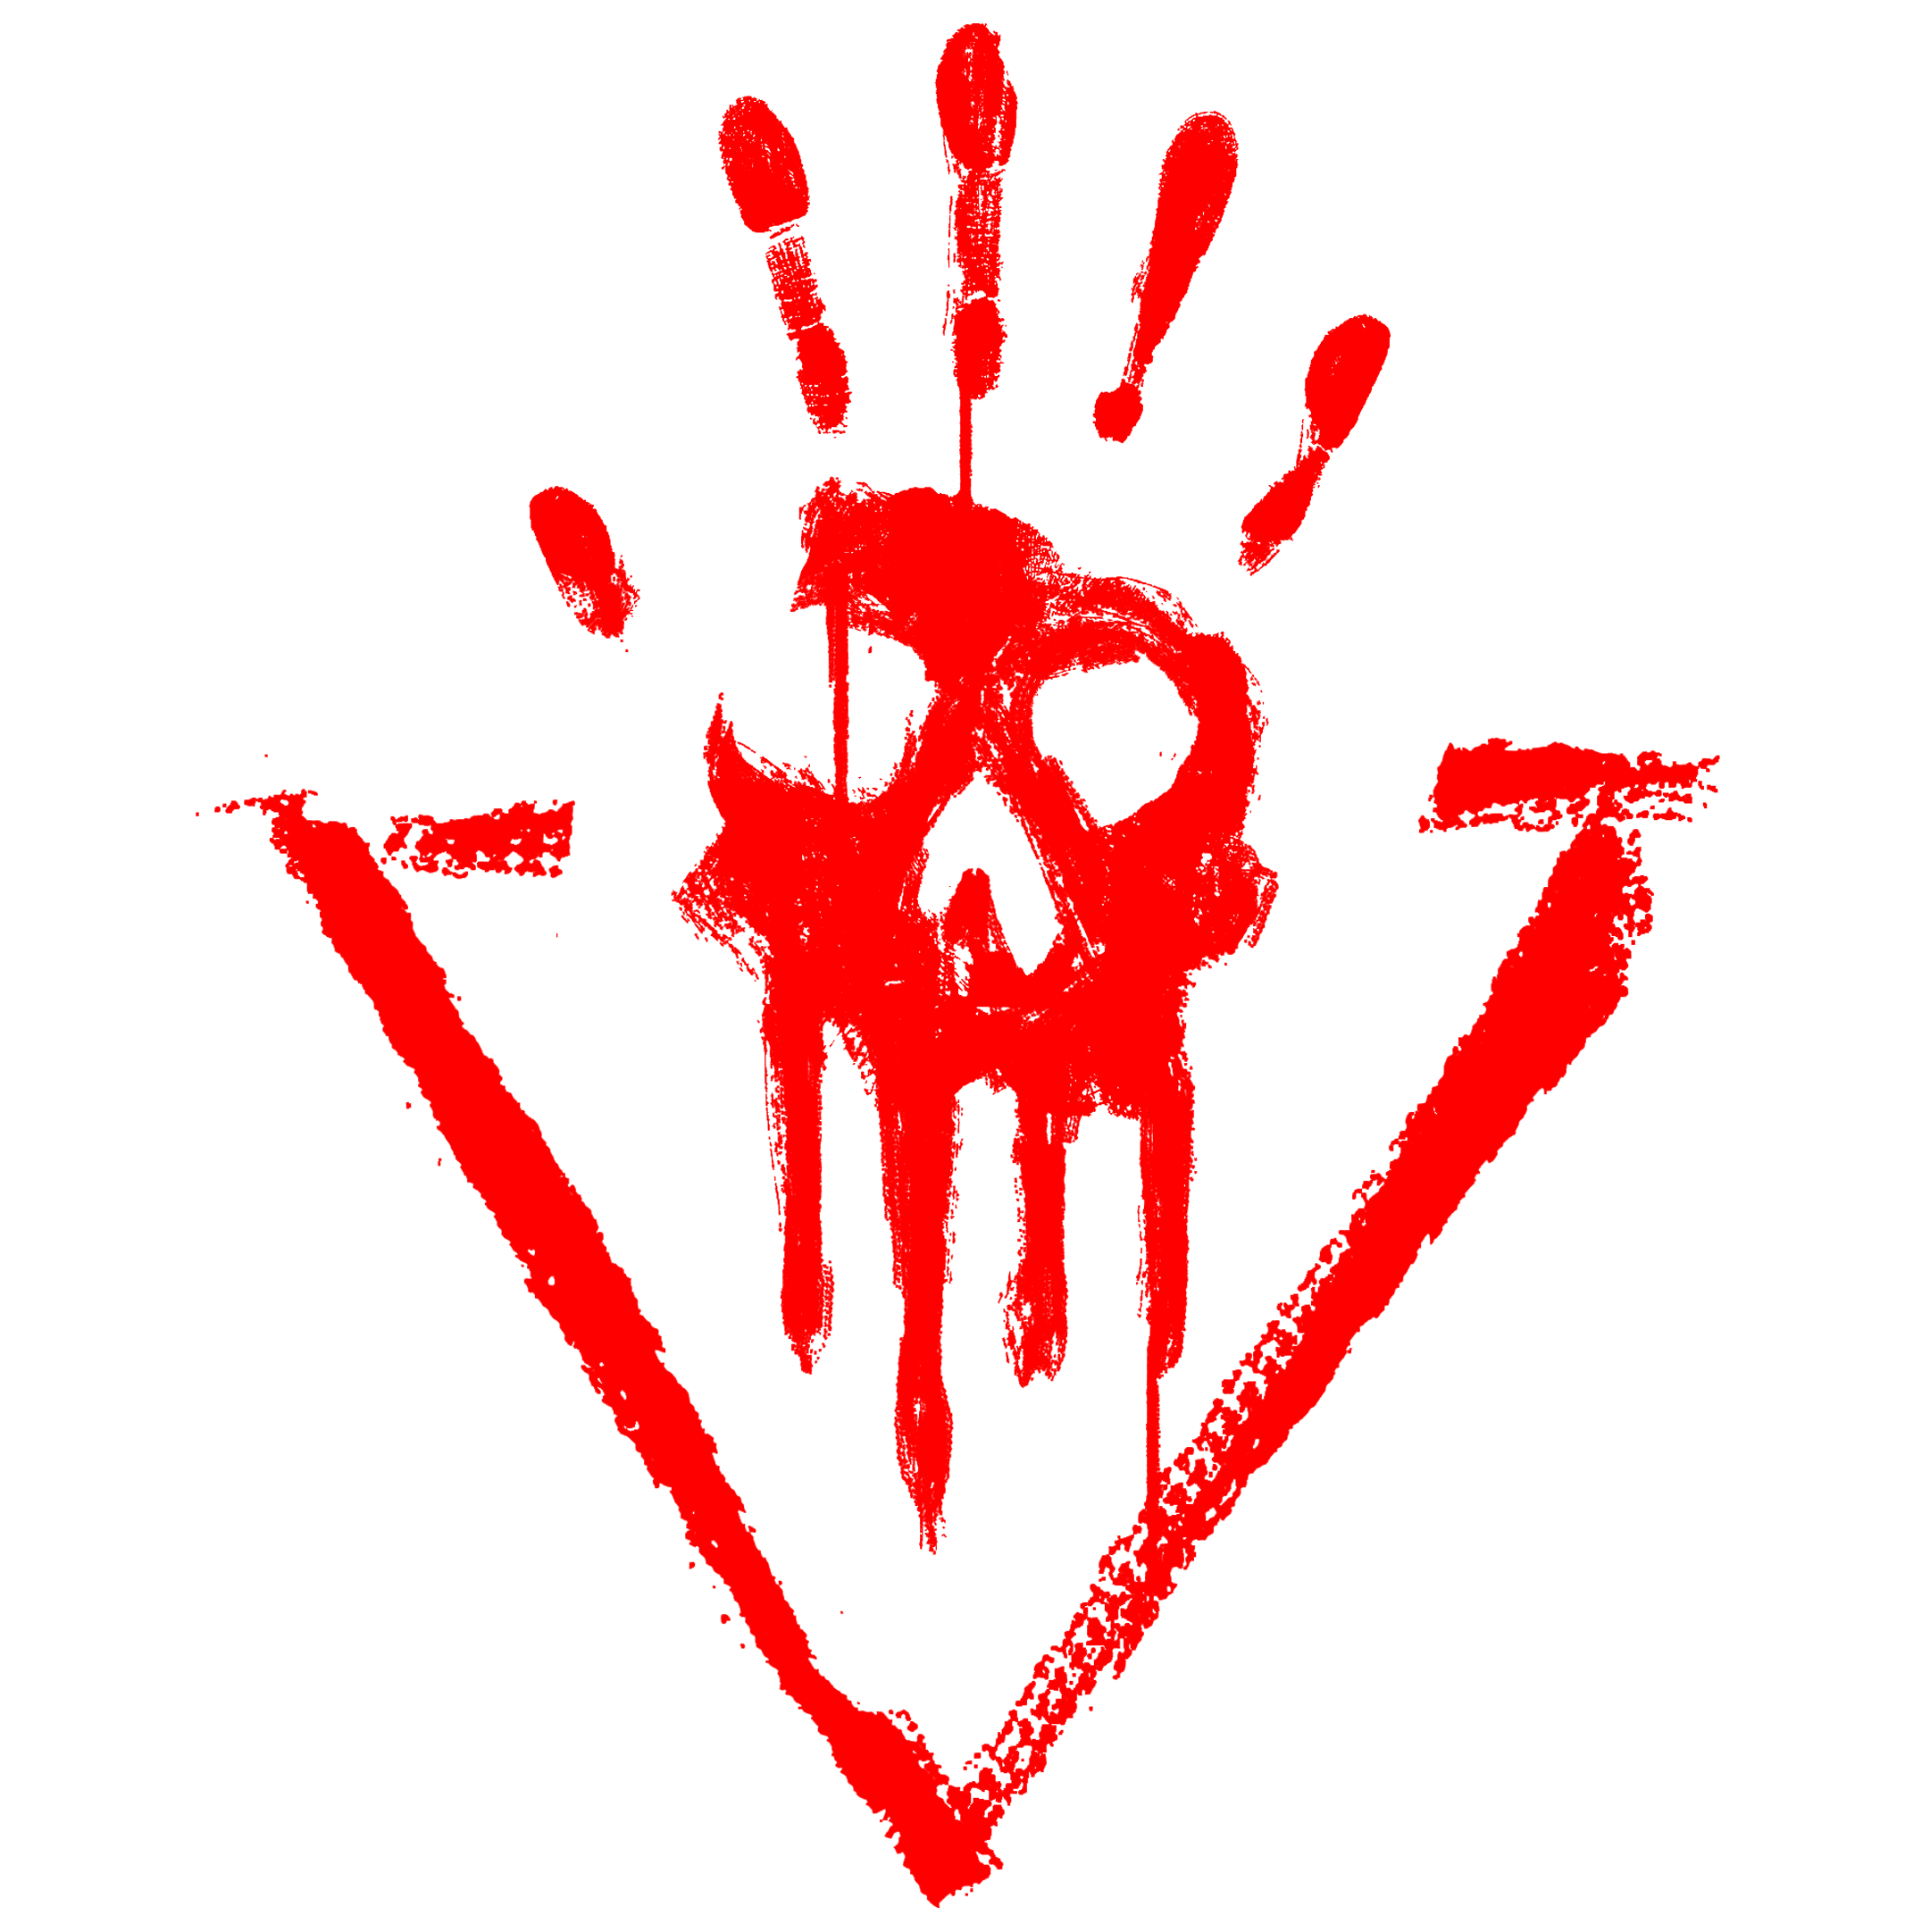
\includegraphics[width=0.12\linewidth]{abs.png}\\
        \vspace{2em}
        \Large\textbf{ITI 1100 Cheat Sheet} \\
        \vspace{0.5em}
        \small{Winter 2024} \\
        \small{University of Ottawa} \\
        \small{Owen Daigle}
    \end{center}

    \pagebreak

    \begin{spacing}{0}
    \tableofcontents
    \end{spacing}

    \pagebreak
    
    % doc begins here

    \section{Number Systems}
    The most important number systems are:
    \begin{itemize}[noitemsep]
        \item Decimal (Base 10): [0,1,2,3,4,5,6,7,8,9]
        \item Binary (Base 2): [0,1]
        \item Octal (Base 8): [0,1,2,3,4,5,6,7]
        \item Hexadecimal (Base 16): [0,1,2,3,4,5,6,7,8,9,A,B,C,D,E,F]
    \end{itemize}

        \subsection{Converting from different bases}
        To convert from decimal to any other base, we will divide the number by the base, and keep track of the remainder. This will be repeated until we get to 0.
        
        To convert from any base to decimal, we use the polynomial notation. This means that the least significant bit (LSB) is assigned a value of $(value)\times (base)^0$, followed by $(value)\times (base)^1$ for the second bit, all the way to $(value)\times (base)^n$ for the most significant bit of an $n$ bit number. 

        \begin{mdframed}
            \textbf{Ex. } Convert the decimal number $73$ into binary, and then back to decimal. 
            \begin{align*}
                &73/2 = 36 +\emph{1}\\
                & 36 / 2 = 18 + \emph{0}\\
                &18/2=9+\emph{0}\\
                &9/2=4+\emph{1}\\
                &4/2=2+\emph{0}\\
                &2/2=1+\emph{0}\\
                &1/2=0+\emph{1}
            \end{align*}
            Then reading from the \emph{bottom up}, we get: $1001001$.

            To go back to decimal, we use the polynomial notation.
            \begin{align*}
                (1001001)_2 = (1\times 2^0 + 0\times 2^1 + 0\times 2^2 + 1\times 2^3 + 0\times 2^4 + 0\times 2^5 + 1\times 2^6)_{10} = 1+8+64 = 73
            \end{align*}
        \end{mdframed}

        To convert to octal or hex, we can take a shortcut by first converting to binary, and then grouping those into 3 (octal) or 4 (hex) bit partitions, and then assigning each of those a corresponding value such as $(011)_2=(3)_8$.

        \begin{mdframed}
            \textbf{Ex. } Convert the binary number $11010110$ into octal. 

            We first group into 3 parts. Note that we can add extra zeroes before the most significant bit (MSB). Then we convert each part to its octal representation. 
            \begin{align*}
                = (011 \text{ } 010\text{ }110)_2 = (326)_8
            \end{align*}
        \end{mdframed}

        To deal with decimals (fractional numbers), we more have to think of this intuitively. 

        We can also use a formula where we multiply the base 10 decimal by the base we want to convert to, and keep only the integer part. Then we repeat using the decimal part again.

        \begin{mdframed}
            \textbf{Ex. } Convert the decimal number 0.375 to binary.
            \begin{align*}
                &0.375\times 2 = \emph{0}.750\\
                &0.750\times 2=\emph{1}.50\\
                &0.50\times 2 = \emph{1}.00
            \end{align*}

            We read from the \emph{top down} and get the value in binary to be 0.011
        \end{mdframed}

        \subsection{Compliments}
        There are 2 types of compliments. 
        \begin{itemize}[noitemsep]
            \item Radix Complement ($r_s$ compliment where $r$ is the base)
            \item Dimished Radix Complement ($(r-1)_s$ compliment where $r$ is the base)
        \end{itemize}

        The radix complement of the base 10 digit 2 is 8.

        The diminished radix complement of a number $n$ is just the radix complement of the number $n$ minus 1. 

        A shortcut with binary to find the 1s compliment is just to flip all 1s to 0s, and all 0s to 1s. If we want the 2s compliment, just add 1 to that. 

        The way to calculate the radix component mathematically is:
        \begin{align*}
            \overline{(N)}_{\text{base}}=(\text{base})^{\text{number of digits in }N}-(N)_{base}
        \end{align*}

        \begin{mdframed}
            \textbf{Ex. } Using the formula, and then the shortcut, find the radix complement of $(101001)_2$.

            We know that the radix complement is the 2s complement. So we can use the formula. 
            \begin{align*}
                \overline{(101001)}_2 = 2^6 - (101001)_2 = 1000000 - 101001 = 010111
            \end{align*}

            The shortcut is only valid for the diminished radix complement (1s complement) but we know that the 2s complement just has 1 added to it. 
            \begin{align*}
                \overline{(101001)}_2 = 010110 + 1 = 010111
            \end{align*}
        \end{mdframed}

        \subsection{Negative Numbers and Subtraction}
        If we are working with signed numbers, then the MSB is not actually the MSB but rather the sign. 1 is negative, 0 is positive. 

        When we are subtracting 2 numbers, $A-B$, we do not actually subtract them. We do $A+2_s(B)$. 

        \begin{mdframed}
            \textbf{Ex. } What is 1001-110101?

            We will need to add the first number with the 2s compliment of the second number. Then we can add them together. 
            \begin{align*}
                2_s(110101) = 001011\\
                \implies 1001+001011 = 010100
            \end{align*}
            We keep the first 0 MSB because we will actually need to get the 2s compliment of this which is $101011+1=101100$.
        \end{mdframed}

    \section{Boolean Algebra}
    When doing boolean algebra, we have access to the following rules:
    \begin{figure}[H]
        \centering
        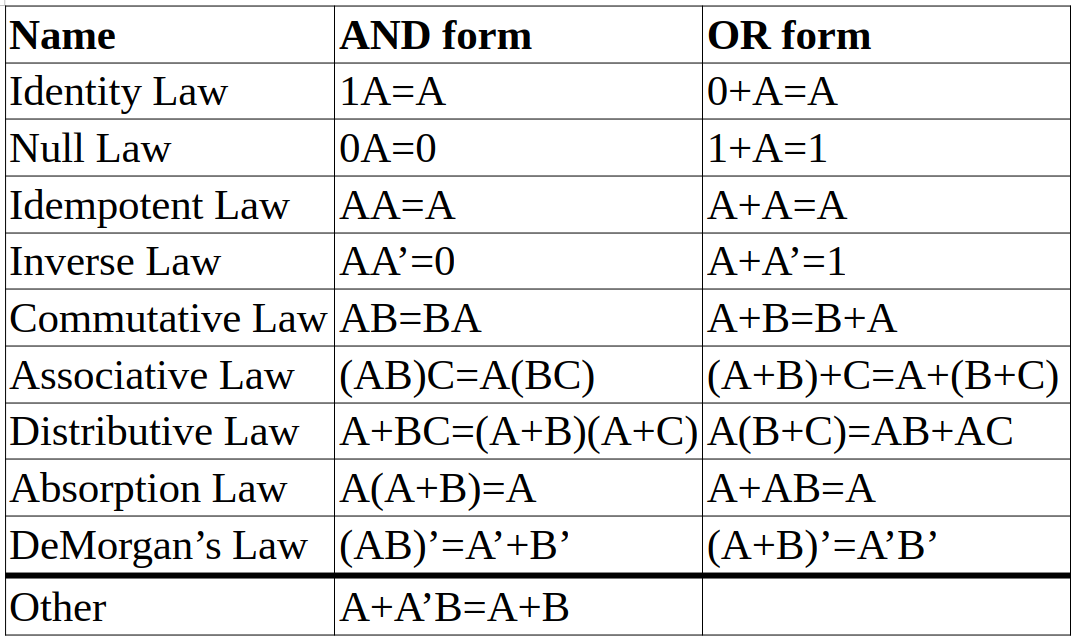
\includegraphics[width=0.6\linewidth]{bol_alg_table.png}
    \end{figure}
    Note that $+$ means or, $\cdot$ means and. 

    We often can create a truth table for a function. This is a table that shows all combinations of inputs and all combinations of outputs.

    \begin{mdframed}
        \textbf{Ex. } Find the truth table for $f(x,y) = x+y$.

        \begin{center}
            \begin{tabular}{ c | c | c }
                x & y & f(x,y) \\
                \hline
                0&0&0\\
                0&1&1\\
                1&0&1\\
                1&1&1
            \end{tabular}        
        \end{center}
        
    \end{mdframed}

        \subsection{Standard Forms}
        To obtain the boolean expressions, we either look for the Sum Of Products (SOP) or the Product Of Sums (POS) forms from the truth table. 

        For the SOP, we look at each row where the output is true, get the state of the input variables in that row and the connect them using AND. We connect all rows using OR. 

        For the POS, we look at each row where the output is false, then get the \emph{complimented} state of all inputs in that row, sum them together, and then take the product of the rows. 

        \begin{mdframed}
            \textbf{Ex. } Find the SOP and POS for the following truth table. 

            \begin{figure}[H]
                \centering
                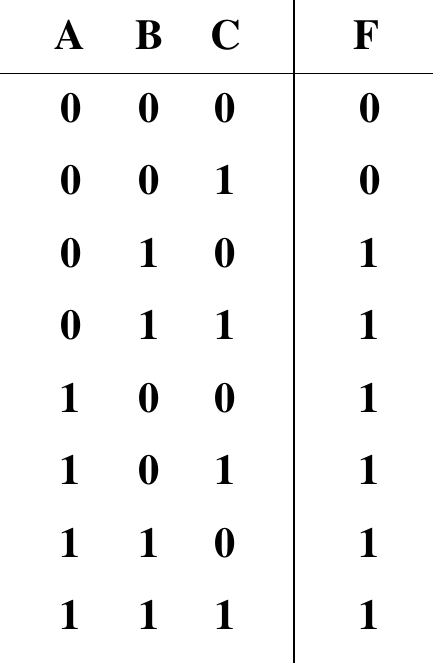
\includegraphics[width=0.2\linewidth]{ex1.png}
            \end{figure}

            For the SOP form, we get all the terms where f is 1. Each of these terms are known as the Minterms. The SOP form is also known as the sum of minterms. 
            \begin{align*}
                F(A,B,C) = \sum m (2,3,4,5,6,7) = A'BC' + A'BC + AB'C' + AB'C + ABC' + ABC
            \end{align*}

            For the POS form, we get all the terms where f is 0. Each of these terms are known as the Maxterms. The POS form is also known as the product of maxterms. 
            \begin{align*}
                F(A,B,C) = \Pi M(0,1) = (A+B+C)\cdot (A+B+C')
            \end{align*}
        \end{mdframed}

        While the SOP and POS forms represent these functions, they are almost always not the most simplified form. We need to use boolean algebra to simplify them. 

        \subsection{Karnaugh Maps (K Maps)}
        The K map is a way to take a truth table and convert it into its \emph{simplest form}.
        
        We take all the rows and put them into a grid. It is a $2\times 3$ grid for 3 variables, or a $4\times 4$ grid for 4 variables. The order we do this is not quite what we expect, but we follow it.

        \begin{figure}[H]
            \centering
            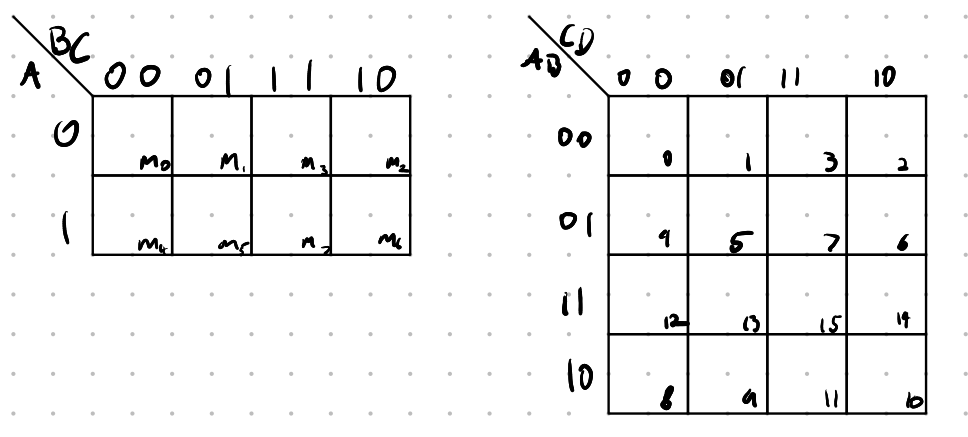
\includegraphics[width=0.6\linewidth]{k1.png}
        \end{figure}

        Then, once we get all the terms in there, we make the biggest groups of 1s possible. These groups contain adjacent squares. These adjacent squares can loop around from one side to the other, or from the top to the bottom. A square can be in multiple groupings.

        \begin{figure}[H]
            \centering
            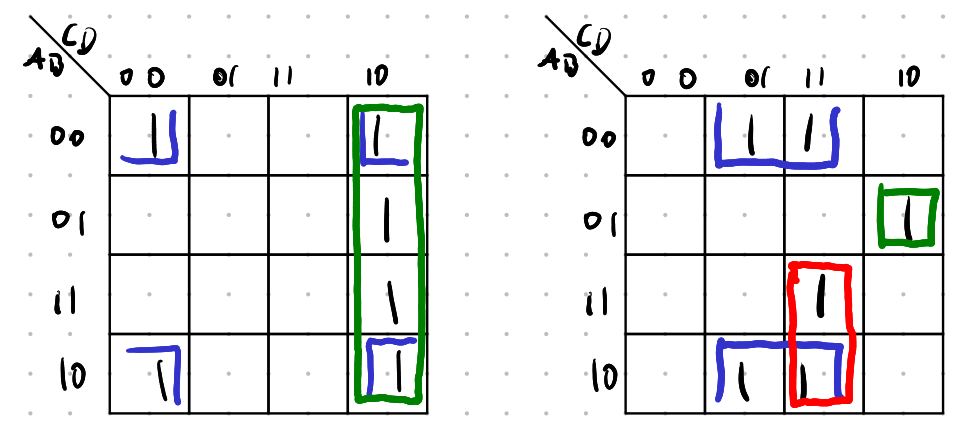
\includegraphics[width=0.6\linewidth]{k2.png}
        \end{figure}

        Then, for each grouping, we will find which variables stay constant in that grouping. Those variables (conjoined with an AND) represents that grouping. Each grouping is connected using an OR. 

        \begin{figure}[H]
            \centering
            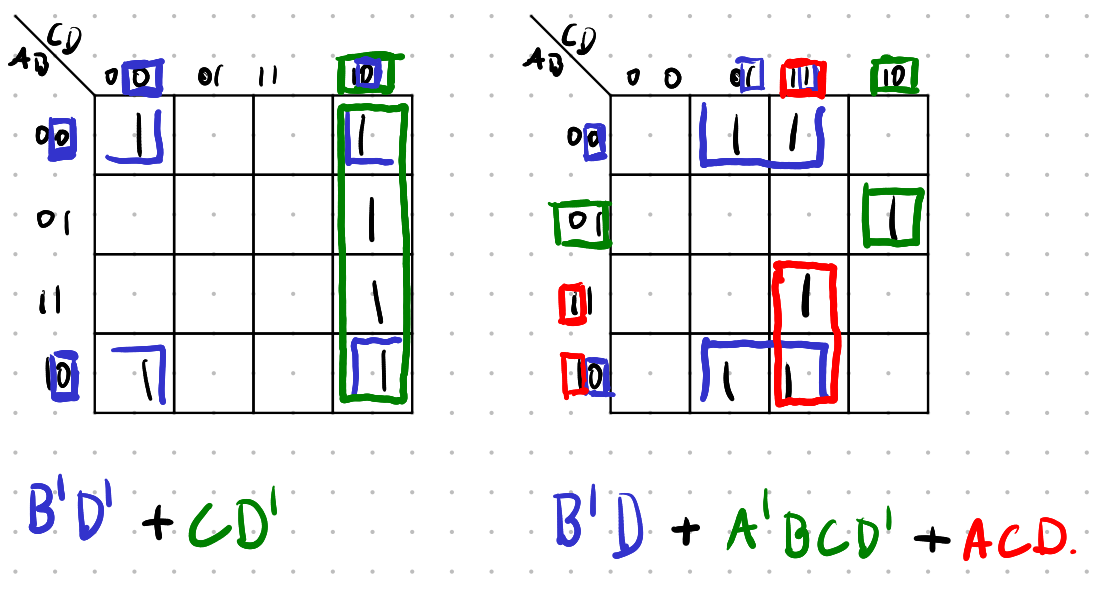
\includegraphics[width=0.6\linewidth]{k3.png}
        \end{figure}

        \begin{mdframed}
            \textbf{Ex. } Find the simplified boolean expression for the following truth table:
            \begin{align*}
                F(w,x,y,z) = \sum m (0,1,2,4,5,6,8,9,12,13,14)
            \end{align*}

            We are not given an explicit truth table, but we are given the sum of minterms. This means each of those minterms (rows) must be 1. 

            Now we can create our k map. We see that we can easily group the left 2 columns, and then for the rightmost column, we can create 2 groups of 4 using the ones from the leftmost column as well. 

            \begin{figure}[H]
                \centering
                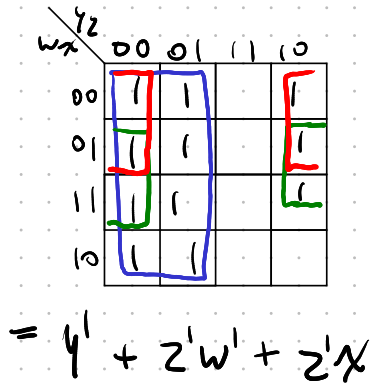
\includegraphics[width=0.3\linewidth]{ex2.png}
            \end{figure}

        \end{mdframed}

        \subsection{Don't Care}
        Don't care conditions are combinations of variables where we don't care about the inputs/outputs. This is often when a certain combination is invalid. 
        
        For example, if we want to convert from binary to decimal on a seven segment display, there are 10 options. 0,1,2,3,4,5,6,7,8,9 which correspond to their binary equivalent. Since there are 10 options, we need 4 input variables. But these 4 input variables have 16 combinations. We will call the combinations 11 through 16 to be invalid, and therefore don't care conditions.

        On the K map, we represent don't cares by an X. This X can be considered \emph{either} a 0 or a 1. We will use whichever gives us the simplest expression. 

        \begin{mdframed}
            \textbf{Ex. } Find the simplified boolean expression for the following k map.

            \begin{figure}[H]
                \centering
                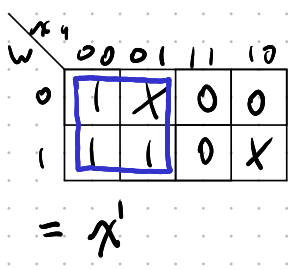
\includegraphics[width=0.3\linewidth]{ex3.png}
            \end{figure}

            Here we will let the don't care at position 001 represent 1, and the don't care at position 110 represent 0. 

            This means that we can consider the whole left 2 columns as 1 group which is just x'.
        \end{mdframed}

    \section{Logic Circuits}
    Logic circuits at their core are made up of OR gates, AND gates, and NOT gates. 

    There are also other gates such as NAND (AND and NOT), NOR (OR and NOT), XOR (Exclusive OR), XNOR (XOR and NOT).

    These are how we show each of them:

    \begin{figure}[H]
        \centering
        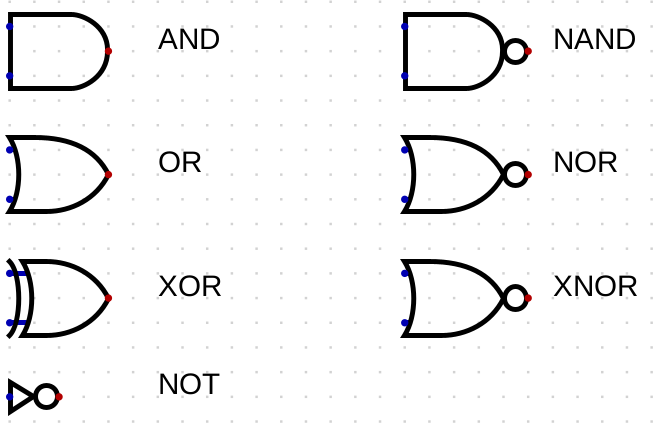
\includegraphics[width=0.4\linewidth]{gates.png}
    \end{figure}

    These gates can also have different number of inputs such as a 4 input AND gate, or a 3 input XOR gate. 

    \begin{mdframed}
        \textbf{Ex. } Draw the circuit diagram of $F(w,x,y,z)=y'+z'w'+z'x$.

        There are many ways to draw this. The most formal way is:
        \begin{figure}[H]
            \centering
            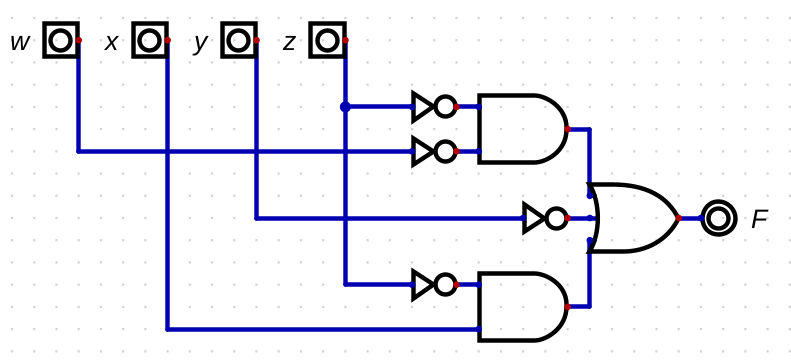
\includegraphics[width=0.65\linewidth]{ex4.png}
        \end{figure}

        An easier way, which is not quite as formal but usually acceptable, allows using complimented inputs, and we can have more than 1 of the same input to simplify things. 
        \begin{figure}[H]
            \centering
            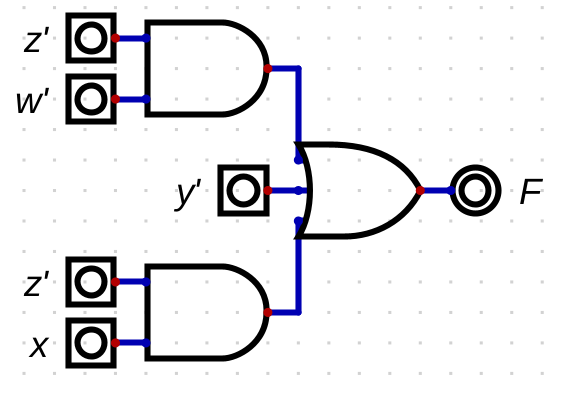
\includegraphics[width=0.34\linewidth]{ex4-2.png}
        \end{figure}

    \end{mdframed}

    \section{Combinatorial Circuits}
    A combinatorial circuit is kind of like a software function. It takes in $n$ inputs, and produces $m$ outputs. This combinatorial circuit can do anything.

    To design one of these, we use the following procedure:
    \begin{enumerate}[noitemsep]
        \item Determine number of required inputs and outputs
        \item Derive truth table
        \item Obtain simplified boolean functions
        \item Draw logic diagram from boolean functions
    \end{enumerate}

    \begin{mdframed}
        \textbf{Ex. } Plan how we would find the circuit diagram for a seven segment display?

        First we would assign each part of the seven segment display a variable. I will use a, b, c, d, e, f, g.

        Then, I will make a truth table with all combinations of inputs (numbers 0-15 in binary) and the corresponding outputs (which sections need to light up on the display). Numbers 10-15 are don't care conditions. 

        Then we get the K maps for each of the outputs a-f.

        Finally, once we have the boolean expressions, we draw the circuit diagram.
    \end{mdframed}
        
        \subsection{Decoders}
        A decoder is a combinatorial circuit that converts $n$ binary inputs into $2^n$ outputs. Basically if the binary number $i$ is the input, then the output is $Q_i$. 
        \begin{figure}[H]
            \centering
            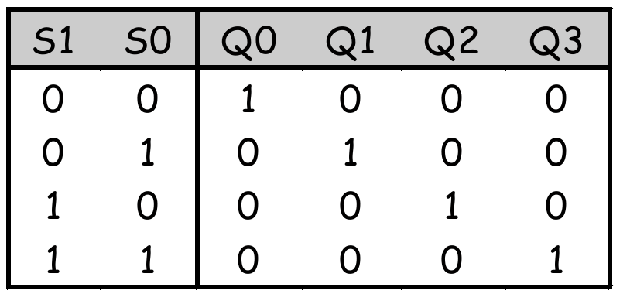
\includegraphics[width=0.3\linewidth]{dec1.png}
        \end{figure}
        
        The input equations are simple, they are just output $Q_i$ written in binary. So output $Q_2$ would have inputs of $S_1S_0'$.

        We can also add an \emph{enabler} input. This input controls whether or not the decoder is enabled. All outputs are 0 iff the enabler is 0. 

        A decoder can be called a minterm or Maxterm generator. This is because it can either generate the minterms or the maxterms of a function. 
        
        The minterm generator is called an active high decoder while the Maxterm generator is called an active low decoder.

        \begin{mdframed}
            \textbf{Ex. } Create the following circuit using 3-8 decoder. $f(x,y,z) = \Pi M(4,5,7)$.

            We know that a 3-8 decoder will have 3 inputs (x,y,z) and 8 outputs (1,7). Since we have the maxterms, we will use the Maxterm generator (Active Low Decoder).

            We will then connect the outputs 4,5,7 to an AND gate. That output will be the function. 
            \begin{figure}[H]
                \centering
                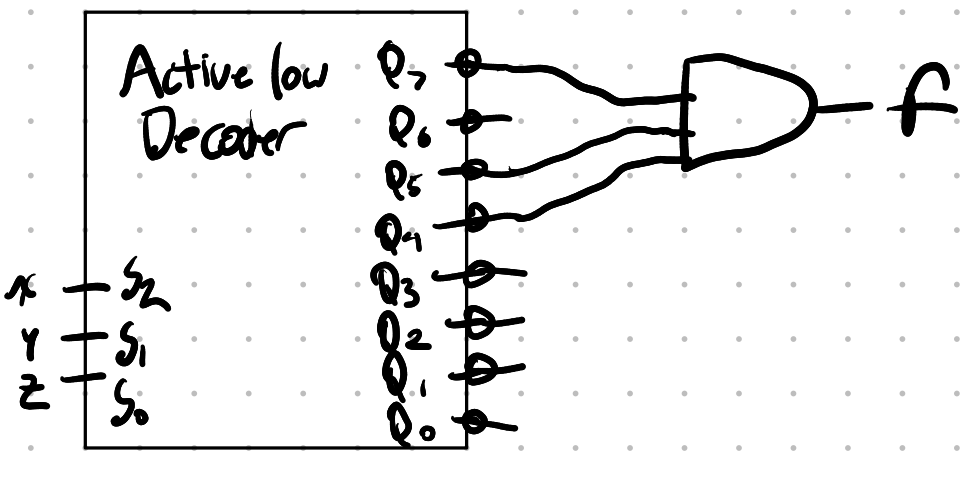
\includegraphics[width=0.4\linewidth]{ex5.png}
            \end{figure}
            Note that the bubbles on the output denote that it is an active LOW decoder. 

            We can also implement this using the minterms. The minterms will be (0,1,2,3,6). So we will connect all of those to an OR gate whose output will be $f$. 
            \begin{figure}[H]
                \centering
                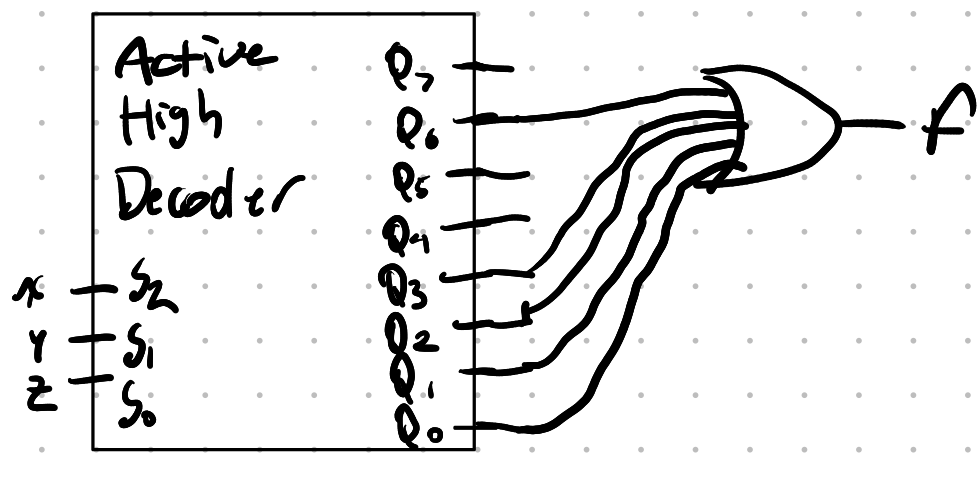
\includegraphics[width=0.4\linewidth]{ex5-2.png}
            \end{figure}
            Note the absence of bubbles on the outputs represent an active HIGH decoder. 
        \end{mdframed}

        \subsection{Encoders}
        An encoder is the opposite of a decoder. It takes in $2^n$ inputs and produces $n$ outputs. 

        We have 2-4 and 3-8 decoders, and we have 4-2 and 8-3 encoders. 

        Since encoders need to only have 1 input active at a time, there are 2 extra steps added to ensure that nothing bad happens. 
        \begin{enumerate}
            \item If 2 or more inputs are equal to 1, the highest numbered position will take precedence. 
            \item We add a Valid output so if the input is all zeroes, then we will set the Valid output to 0.  
        \end{enumerate}

        \subsection{Multiplexers (MUX)}
        A MUX is basically a data selector. We have multiple inputs, and one output. The output takes the value of one of the input lines depending on the value of the \emph{selector bits}. 

        We can implement functions using MUXs. We do this by treating the input variables as the selectors, and then treating the input lines as the minterms. If the minterm is a 1, then we feed a logic 1. Otherwise, we feed nothing. 

        \begin{mdframed}
            \textbf{Ex. } Inplement the following function using a MUX: $f(x,y,a) = \sum m (1,2,6,7)$.

            First we create a truth table to visualize the function. 
            \begin{figure}[H]
                \centering
                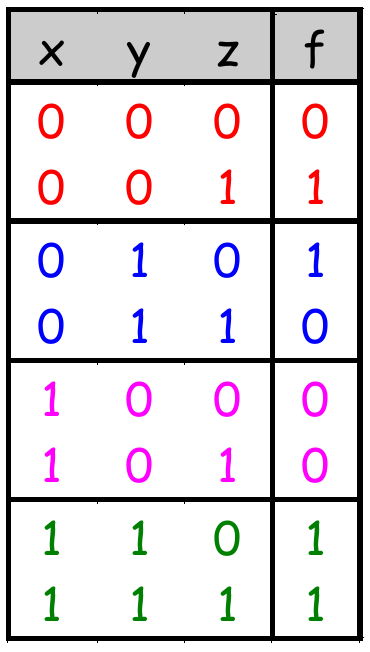
\includegraphics[width=0.15\linewidth]{ex6.png}
            \end{figure}

            We will create an 8-1 MUX using the inputs x,y,z as selectors. For the inputs, we will feed 1 into 1,2,6,7 since those are the minterms (rows in which f is 1).
            \begin{figure}[H]
                \centering
                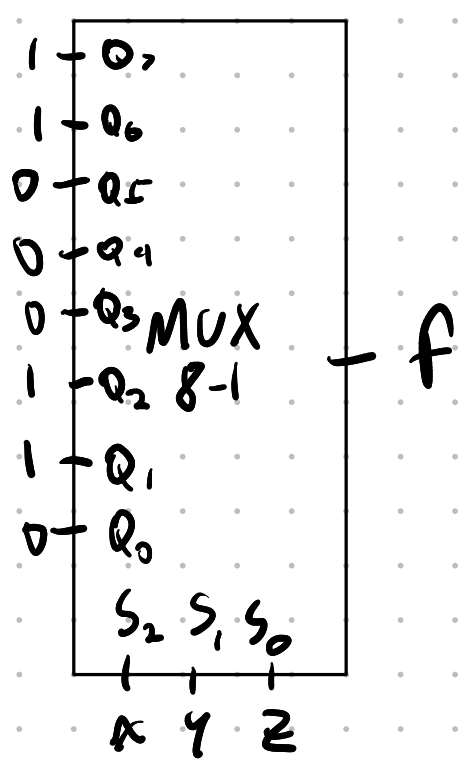
\includegraphics[width=0.2\linewidth]{ex6-2.png}
            \end{figure}

            We can also make this using a 4-1 MUX by observing that the $z$ input and the output are related. For the first 2 rows (when $x=y=0$) $f=z$. For the next 2, $f=z'$. For the next 2, $f-0$, and for the last 2, $f=1$. We can feed this directly into the 4-1 decoder.
            \begin{figure}[H]
                \centering
                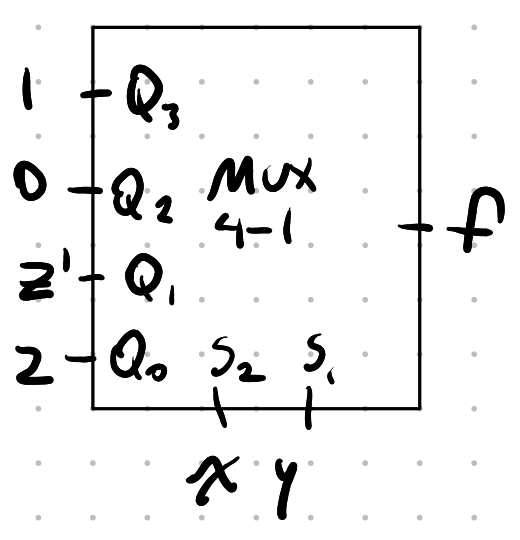
\includegraphics[width=0.2\linewidth]{ex6-3.png}
            \end{figure}
        \end{mdframed}

    \section{Sequential Circuits}
    A sequential circuit is a circuit that has knowledge of the history of the circuit (memory). These circuits may operate differently depending on what the circuit was doing previously. 

    For example, an elevator needs to remember what floor it is on. If you click on the "Floor 2" button, if it is currently on floor 1, it needs to go up, but if it is currently on floor 3, it needs to go down. 

    So there are both \emph{inputs}, and the \emph{previous states} that we need to deal with. 

    These circuits can be either \emph{asynchronous}, or \emph{synchronous}. Synchronous means that it will only trigger when a clock pulses. Asynchronous means that it will trigger as soon as possible. 

    For the synchronous, it can either be \emph{positive transition}, or \emph{negative transition}. Positive transition is when the clock was just at 0, and is turning to 1, Negative transition is when the clock was just at 1, and is turning to 0. 

    \begin{figure}[H]
        \centering
        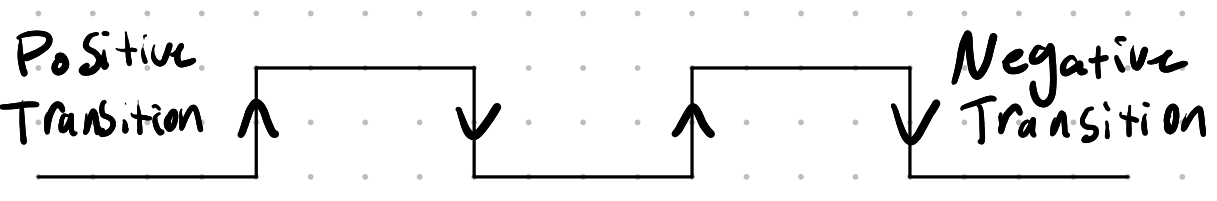
\includegraphics[width=0.7\linewidth]{pos-neg-trans.png}
    \end{figure}

        \subsection{Latches}
        Latches are asynchronous memory elements. They can store 1 bit of data. 

        The SR latch is a latch with the following truth table. Note that $Q_t$ is the current time, $Q_{t+1}$ is the next time. 
        \begin{center}
            \begin{tabular}{ c | c | c}
                S & R & $Q_{t+1}$ \\
                \hline
                0&0&$Q_t$\\
                0&1&0\\
                1&0&1\\
                1&1&UNKNOWN
            \end{tabular}        
        \end{center}
        The unknown state is bad. We never want to get that state. 

        There is also the D latch. This one is much simpler.
        \begin{center}
            \begin{tabular}{ c | c }
                D&$Q_{t+1}$\\
                \hline
                0&0\\
                1&1
            \end{tabular}        
        \end{center}

        \subsection{Flip Flops}
        Flip Flops are very similar to latches except they have a clock input as well. They do not change their state even if the inputs change, until the clock pulses (either negative or positive transition)

        Generally we have the following flip flops:
        \begin{itemize}[noitemsep]
            \item D Flip Flop (Same as D latch except with a clock)
            \item JK Flip Flop (Same as SR latch except with a clock and undefined state becomes a toggle state. J=set, K=reset)
            \item T flip flop (Toggle Flip Flop, 1 is toggle, 0 is same state)
        \end{itemize}

        We often make state tables to deal with flip flops. These are tables with the inputs, the present states, the next states, and the outputs if applicable. 

        \begin{mdframed}
            \textbf{Ex. } Come up with the state table for the following sequential circuit with 2 D flip flops. 
            \begin{figure}[H]
                \centering
                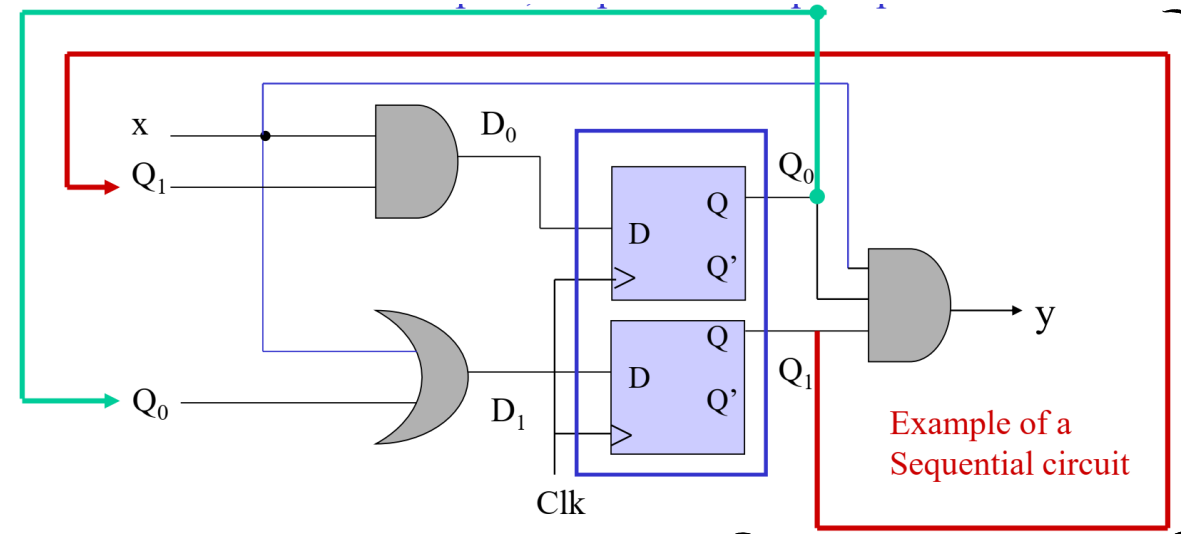
\includegraphics[width=0.5\linewidth]{f1.png}
            \end{figure}

            We know that it needs to have all 4 combinations for the present state. Since the next state depends on $x$ as well, we either need to create 8 rows in total in the table, or have different next state columns depending on $x$. I will have different next state columns. We also need to show the output of $x$, again depending on the previous $x$ value. 
            \begin{figure}[H]
                \centering
                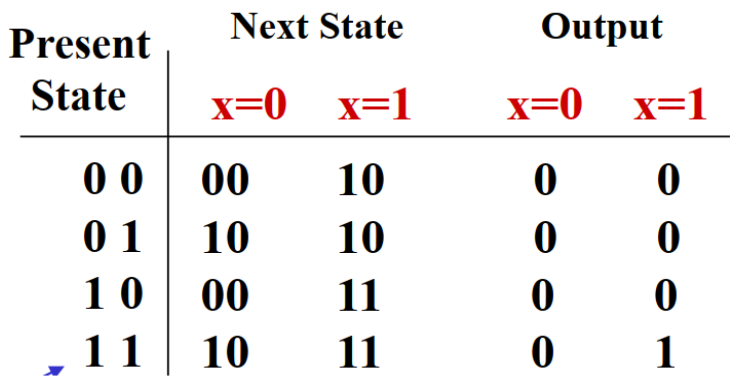
\includegraphics[width=0.3\linewidth]{f2.png}
            \end{figure}

            The state diagram is a way to visually represent this. Here is the state diagram for this example. 

            This shows where each state goes depending on the next state (shown by the arrows), and the value of $x$ (shown by the first number above the arrow). The next value of $x$ is shown by the second number above the arrows. 
            \begin{figure}[H]
                \centering
                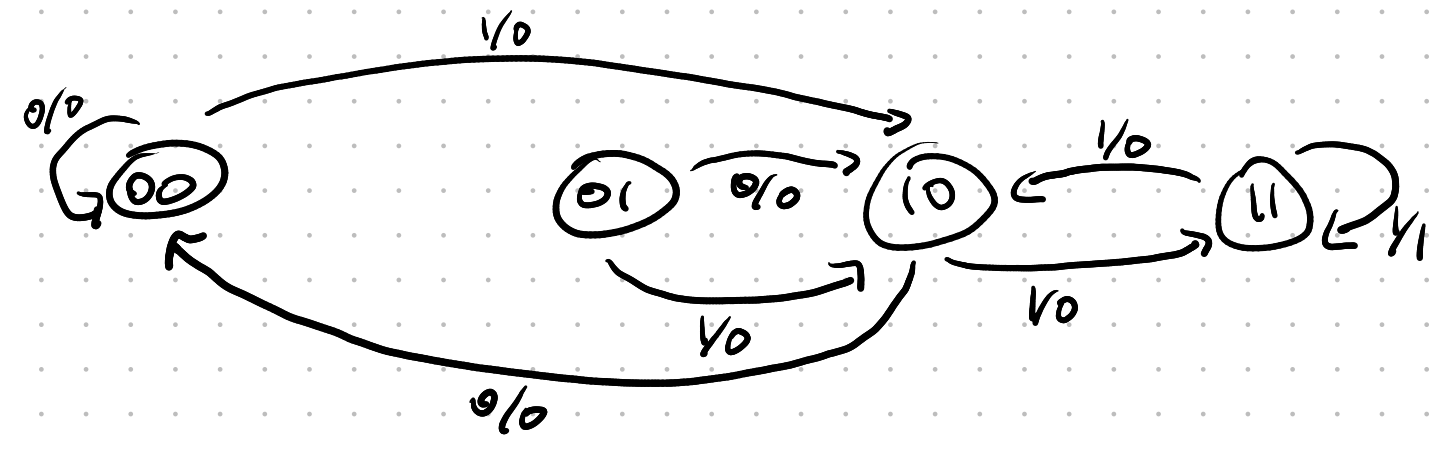
\includegraphics[width=0.6\linewidth]{f3.png}
            \end{figure}
        \end{mdframed}
        

        We also use transition tables (Excitation tables) for each type of flip flop. These show us what inputs we need to go from one state to another state. 
        \begin{figure}[H]
            \centering
            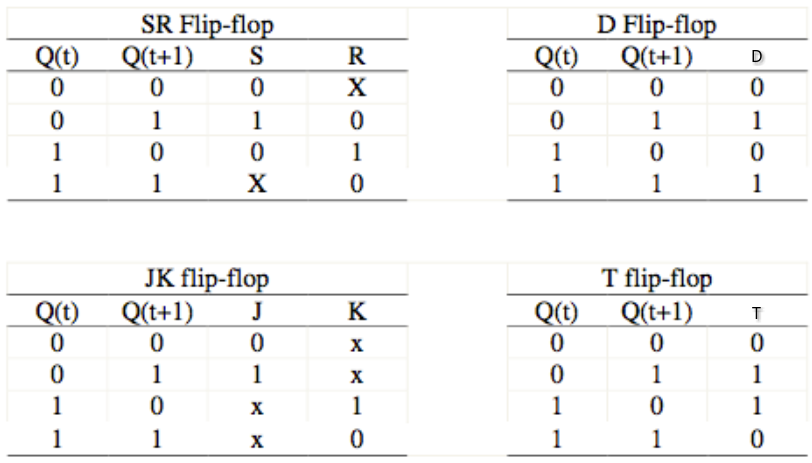
\includegraphics[width=0.55\linewidth]{excitation.png}
        \end{figure}

        \subsection{Circuit Design}
        To design a circuit, we follow this procedure:
        \begin{enumerate}
            \item Obtain state diagram either directly, or from word description. 
            \item Reduce number of states if possible. 
            \item Assign binary codes to states.
            \item Choose type of flip flop
            \item Derive flip flop input equations
            \item Draw circuit diagram
        \end{enumerate}

        \begin{mdframed}
            \textbf{Ex. } Design a sequential circuit that will detect a series of 3 or more consecutive ones.

            We need to obtain the state diagram.
            \begin{itemize}[noitemsep]
                \item State 0: Detected 0 consecutive ones (output = 0)
                \item State 1: Detected 1 consecutive ones (output = 0)
                \item State 2: Detected 2 consecutive ones (output = 0)
                \item State 3: Detected 3 consecutive ones (output = 1)
            \end{itemize}
            The state diagram and tables look like this.
            \begin{figure}[H]
                \centering
                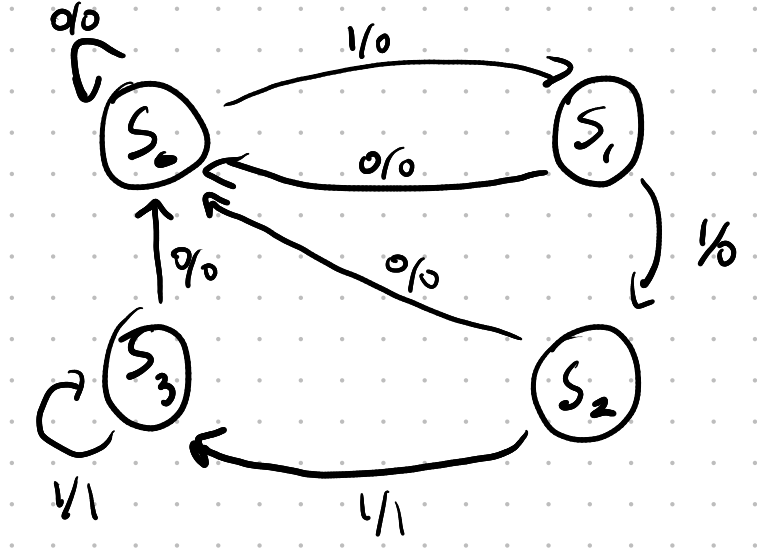
\includegraphics[width=0.3\linewidth]{ex9.png}
            \end{figure}
            \begin{figure}[H]
                \centering
                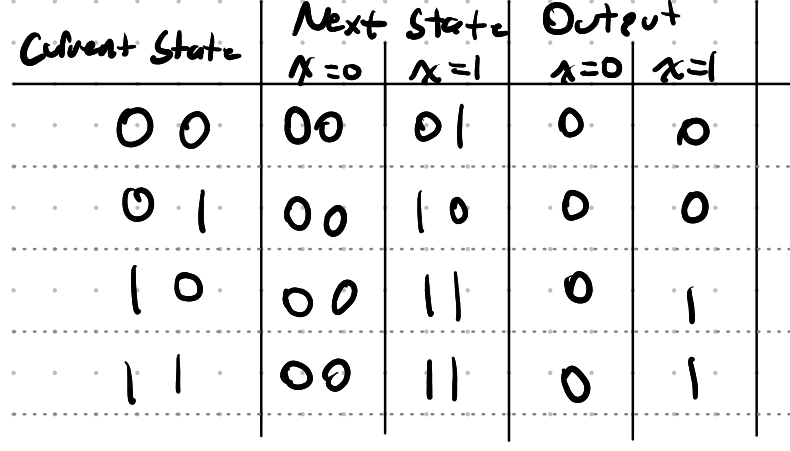
\includegraphics[width=0.4\linewidth]{ex9-2.png}
            \end{figure}
            We will then choose to go with D flip flops as they are easy to work with. I will give them the names of A and B. 

            I will also call the output y.

            I will create a bigger state table with the states seperated into A and B, $A-{t+1}$ and $B_{t+1}$, and then add on the columns for the input to $D_A$ and $D_B$. This is found through the D flip flop excitation table. 
            \begin{figure}[H]
                \centering
                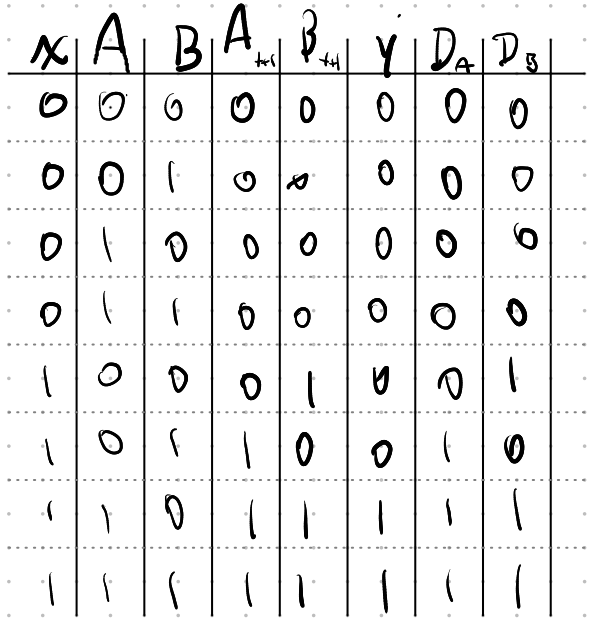
\includegraphics[width=0.4\linewidth]{ex9-3.png}
            \end{figure}

            Now I can get the equations for the D flipflop inputs A and B, and the output y. I will use K maps to get:
            \begin{align*}
                D_A = xA + xB\\
                D_B = xB' + xA\\
                y = xA
            \end{align*}

            Now I can finally draw the circuit. 
            \begin{figure}[H]
                \centering
                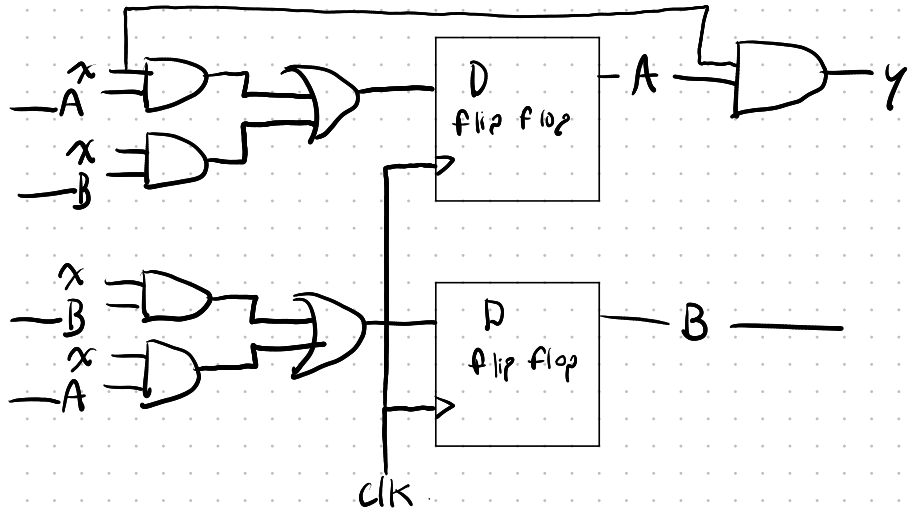
\includegraphics[width=0.8\linewidth]{ex9-4.png}
            \end{figure}
        \end{mdframed}

        \subsection{Counters}
        A counter is simply a circuit that counts. It does not have to count from 0 to n, it can count in a weird order such as 001, 010, 101, 011, 000. We can easily build these counters. 

        \begin{mdframed}
            \textbf{Ex. } Build a counter that counts from $0\to 3\to 5\to 7\to 6\to 0$

            First we start with the state diagram. We notice that we are missing a few states, but that is not a problem. They will just be considered don't cares. 
            \begin{figure}[H]
                \centering
                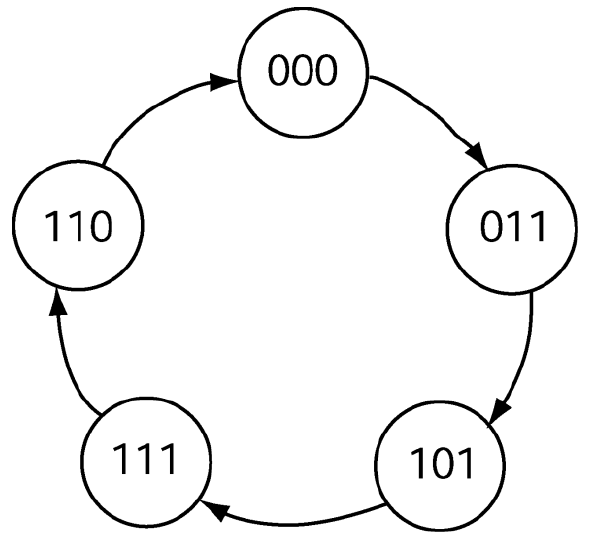
\includegraphics[width=0.2\linewidth]{ex7.png}
            \end{figure}

            Then we do the state table. We know what the present states and next states will be. For example, if the present state is 0 = 000, then the next state is 3 = 011. If the present state is 001, well this is not possible so we don't care about the next state. 

            For the flip flop inputs, we will use the JK excitation table. For $J_A$, we see that A goes from a 0 to a 0. This corresponds to J of 0, and K of X. We do this for each of the flip flop inputs for each of the states. 
            \begin{figure}[H]
                \centering
                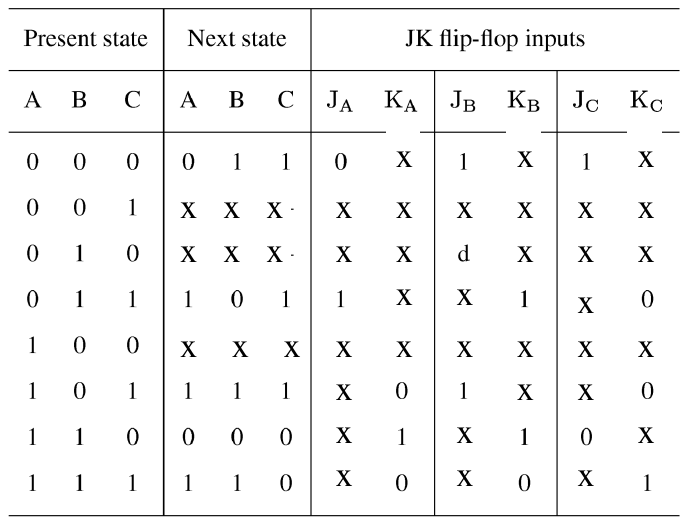
\includegraphics[width=0.6\linewidth]{ex7-2.png}
            \end{figure}

            Now we basically have the truth table. So we need to get the equations for $J_A, K_A, J_B, K_B, J_C, K_C$. We use the K maps for those. 

            The rest is very straight forward. We get the equations, and then we use that to build the circuit. 

            For $J_A$, we end up getting B. Note that B  means the output from the flip flop B. 
            \begin{figure}[H]
                \centering
                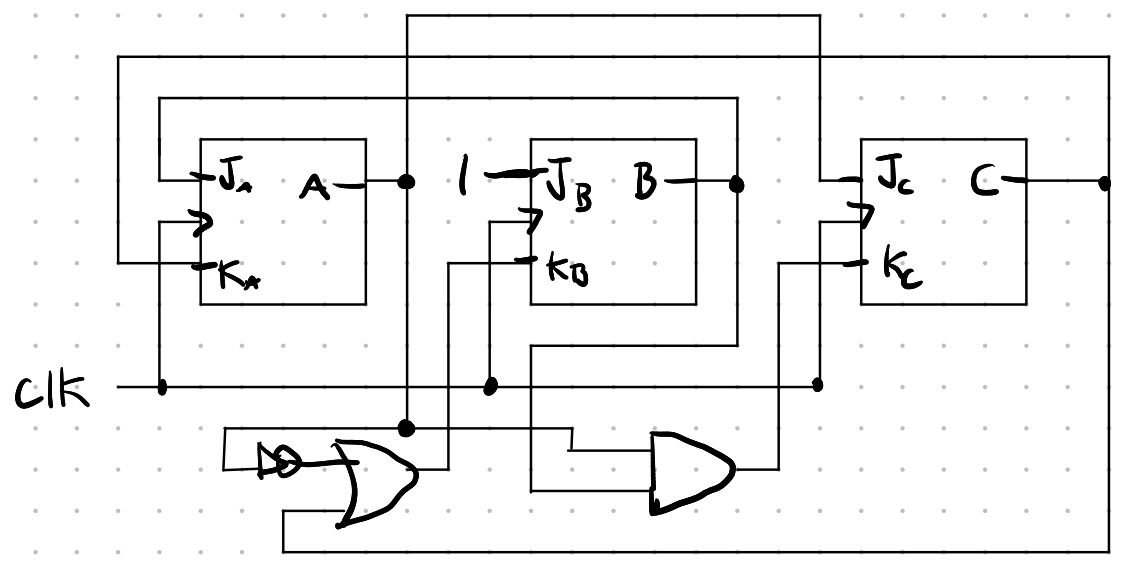
\includegraphics[width=0.7\linewidth]{ex8.png}
            \end{figure}
            This ends up being very complicated, so we usually remove all the lines and just state the inputs. 
            \begin{figure}[H]
                \centering
                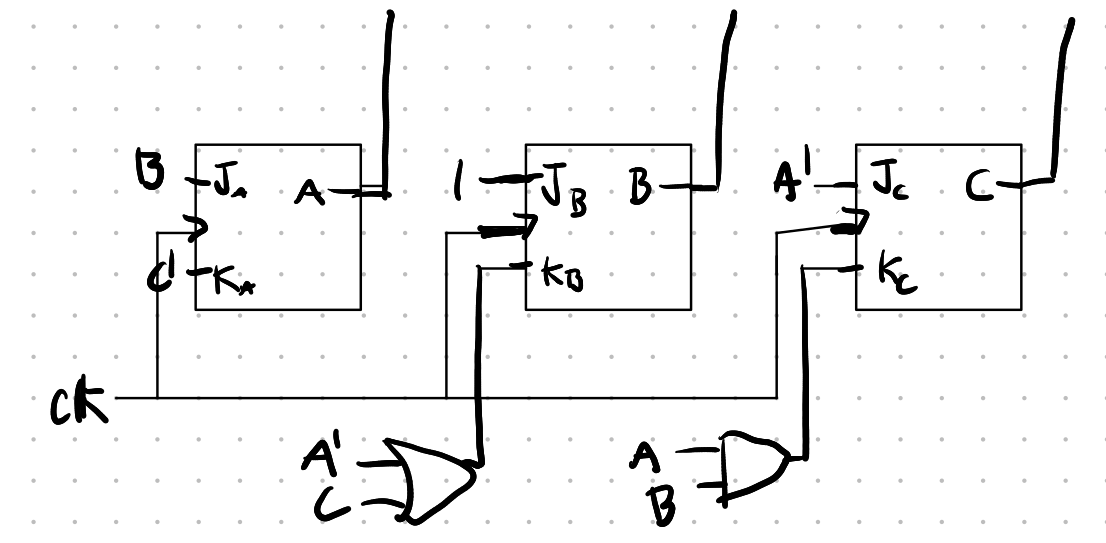
\includegraphics[width=0.6\linewidth]{ex8-2.png}
            \end{figure}

        \end{mdframed}  

\end{document}